\documentclass[../main.tex]{subfiles}




\begin{document}







\chapter{Propietats de separació}
\section{Espais topològics separables}

\begin{defi}[Espai topològic separable]
\label{def:espaitopologicseparable}\index{Espai topològic separable} Sigui $(X,\tau)$ un espai topològic. Aleshores $X$ es diu \textit{separable} si conté un subconjunt dens i numerable.
\end{defi}

\begin{ej}
\label{ej:separable1} Considerem l'espai topològic $(\mathbb{R},\tau)$ amb la topologia $\tau$ usual. Recordem que $\mathbb{Q}$ és dens a $\mathbb{R}$, (\ref{ej:qesdensar}). Això és perquè qualsevol obert de $\mathbb{R}$ és o bé $\emptyset$, o bé una unió d'una col·lecció arbitrària d'intervals oberts i tot interval obert conté un racional. Per tant, la intersecció de qualsevol obert de $\mathbb{R}$ amb $\mathbb{Q}$ és no buida.

A més, el conjunt dels racionals és numerable. Per tant, $\mathbb{Q}$ és un subconjunt dens i numerable i per tant $\mathbb{R}$ és un espai topològic separable.
\end{ej}

\begin{ej}
\label{ej:separable1} Considerem $\mathbb{R}$ amb la topologia $\tau = \{[a,b)\;:\;a,b\in\mathbb{R},\;a<b\}$. Volem determinar si $(\mathbb{R},\tau)$ és un espai topològic separable. Veiem que $\mathbb{Q}$ també és dens en aquesta topologia.

En efecte, sigui $U\in\tau\setminus\{\emptyset\}$. Aleshores $U$ és una d'aquestes dues opcions
\begin{equation}
    \notag
    U = \left\{
    \begin{array}{lcl}
        \left[a,b\right) & \text{per a alguns} & a,b\in\mathbb{R},\;a<b \\
        \text{unió d'intervals}\;\left[a,b\right) & \text{per a alguns} & a,b\in\mathbb{R},\;a<b;
    \end{array}
    \right.
\end{equation}
i en qualsevol cas $[a,b)\subseteq U$ per a alguns $a,b\in\mathbb{R}$, $a<b$. Aleshores, per certs $a,b\in\mathbb{R}$, suposem que $\mathbb{Q}\cap U=\emptyset$. Això implica que $\mathbb{Q}\cap [a,b) = \emptyset$. Però això diu aleshores que $\forall x$ tal que $a\leq x<b$, $\not\exists q\in\mathbb{Q}$ tal que $a\leq x<q<b$. Però sabem que, donat qualsevol $x\in [a,b)$ sempre existeix un racional $q\in\mathbb{Q}$ tal que $x<q<b$ i això aleshores és una contradicció, ergo $\mathbb{Q}\cap U\not=\emptyset$, $\forall U\in\tau\setminus\{\emptyset\}$.
\end{ej}

\begin{ej}
\label{ej:3} Construir una topologia $\tau$ a $X = \{a,b,c,d\}$ tal que $(X,\tau)$ sigui separable. Considerem la topologia
\begin{equation}
    \notag
    \tau = \{\emptyset,\{a\},\{b\},\{a,b\},\{a,b,c\},X\}. 
\end{equation}
Clarament cada subconjunt de $X$ és numerable ja que $X$ és numerable. Aleshores només queda trobar-ne un de dens.

Considerem $A = \{a,b\}\in\tau$. Aleshores, tenim
\begin{equation}
    \notag
    A\cap\{a\} = \{a\}\not=\emptyset,\quad A\cap\{b\}=\{b\}\not\emptyset,\quad,\cdots,\quad A\cap X = \{a,b\}\not=\emptyset.
\end{equation}
i així $A$ és un subconjunt dens i numerable, ergo $(X,\tau)$ és un espai topològic separable.
\end{ej}

\begin{prop}
[Exemple]\label{prop:separable1} Si $X$ és un conjunt finit i $\tau$ la topologia discreta en $X$, aleshores l'espai topològic $(X,\tau)$ és separable
\end{prop}
\begin{proof}
Sigui $X$ un conjunt finit amb $n$ elements. Posem $X = \{a_1,\ldots,a_n\}$. Si $\tau$ és la topologia discreta, aleshores $\tau = \mathscr{P}(X)$. Clarament tot subconjunt de $X$ és numerable, ja que $X$ és numerable. Per tant, només cal trobar un subconjunt dens de $X$. Prenent $A = X$, $\forall U\in\tau\setminus\{\emptyset\}$ es compleix que $U\subseteq A$ i per tant $U\cap A = U\not=\emptyset$. Per tant $A$ és numerable i dens en $X$ i per tant $(X,\tau)$ és separable.
\end{proof}

\begin{prop}[Exemple]
\label{prop:separable2} Si $X$ és un conjunt numerable i $\tau$ la topologia discreta, aleshores l'espai topològic $(X,\tau)$ és separable.
\end{prop}
\begin{proof}
Si $X$ és numerable, aleshores és o bé finit, o bé infinit i numerable. Si $X$ és finit, ja ho hem demostrat a (\ref{prop:separable1}). Suposem doncs que $X$ és un conjunt infinit i numerable. Sigui $X = \{a_1,a_2,\ldots\}$. Prenent $A = X$ obtenim que $\forall U\in\tau\setminus\{\emptyset\}$ és tal que $U\subseteq A$ i així doncs $A\cap U = U\not=\emptyset$. Per tant $A$ és numerable i dens, ergo $(X,\tau)$ és separable.
\end{proof}

\begin{ter}
\label{ter:numerableimplicaseparable} Sigui $(X,\tau)$ un espai topològic. Si $X$ és numerable, aleshores $(X,\tau)$ és un espai topològic separable.
\end{ter}
\begin{proof}
Sigui $X$ un conjunt numerable i $\tau$ qualsevol topologia en $X$. Per definició, $\tau$ conté $X$. Aleshores, si prenem $A = X$ ja es compleix que $A$ és numerable (trivial) i dens, ja que $\forall U\in\tau\setminus\{\emptyset\}$ tenim que $U\subseteq A$ i per tant $U\cap A = U\not=\emptyset$. Per tant, $(X,\tau)$ és separable.
\end{proof}

\section{Espais topològics de Kolmogorov}

\begin{defi}
[Espai topològic de Kolmogorov]\label{def:kolmogorov}\index{Espai topològic de Kolmogorov}\index{Kolmogorov} Un espai topològic $X$ es diu que és $T_0$ o de \textit{Kolmogorov} si per tot parell de punts diferents $x,y\in X$, $x\not=y$, existeixen entorns oberts $U_x$ de $x$ i $U_y$ de $y$ tals que o bé $y\not\in U_x$, o bé $x\not \in U_y$.
\end{defi}

Gràficament:
\begin{equation}
    \notag
    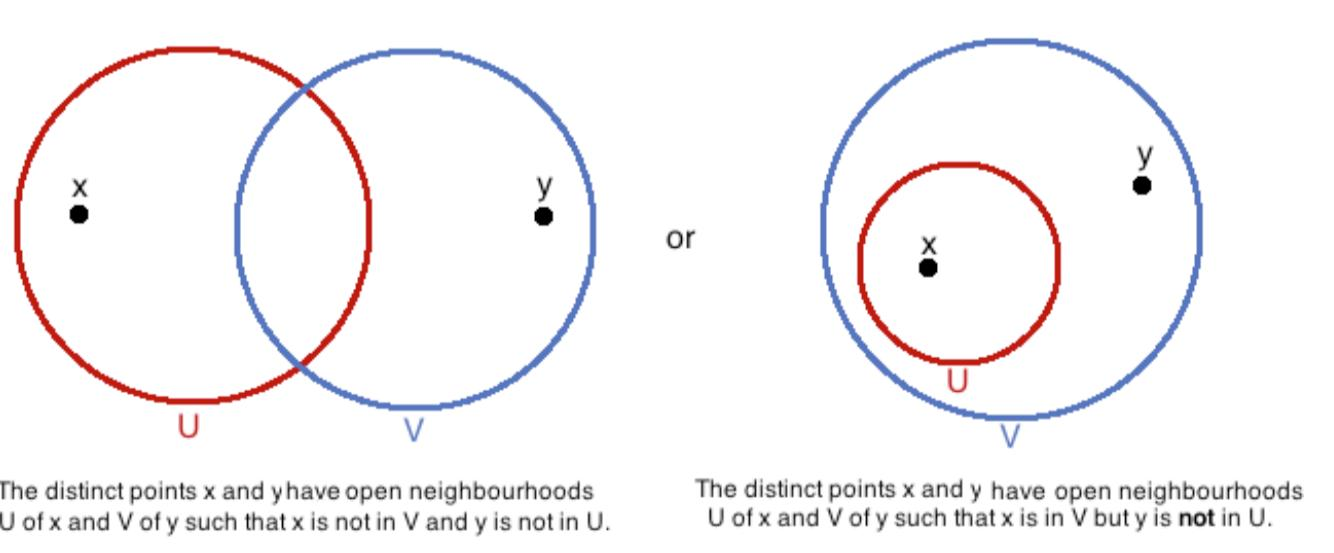
\includegraphics[scale = 0.3]{fotos_topo_1/t0.jpeg}
\end{equation}
Aquesta és la forma més feble de separació.

\begin{ej}
\label{ej:kolmogorov} Sigui $X = \{a,b,c,d\}$ i sigui $\tau_g$ la topologia grollera a $X$, $\tau_g = \{\emptyset,X\}$. Aleshores $(X,\tau_g)$ no és $T_0$ perquè si dos punts diferents $x,y\in X$, els únics entorns oberts són el total per als dos.
\end{ej}

\begin{prop}
\label{prop:kolmogorov} Un espai topològic és $T_0$ o de Kolmogorov si, i només si, per tot parell de punts diferents $x,y\in X$, $x\not=y$, existeix un obert $U$ que conté només un dels dos, $x$ o bé $y$.
\end{prop}
\begin{proof}
Suposem que $X$ és $T_0$ i siguin $x,y\in X$, $x\not=y$. Aleshores existeixen entorns oberts $U$ de $x$ i $V$ de $y$ tals que o bé $x\not\in V$ o bé $y\not \in U$. Si $x\not\in V$, aleshores $V$ és un obert que només conté a $y$. Si $y\not\in U$, aleshores $U$ és un obert que només conté a $x$. Així obtenim el que volíem.

Recíprocament, suposem que per a tot parell $x,y\in X$, $x\not=y$, $\exists U$ obert tal que només un dels dos elements està a $U$. Suposem, sense pèrdua de generalitat, que $x\in U$ només. Aleshores $U$ és un entorn obert de $x$ que no conté a $y$, ergo $X$ és $T_0$.
\end{proof}

\section{Espais topològics de Fréchet}

\begin{defi}
[Espai de Fréchet]\label{def:frechet}\index{Fréchet}\index{Espai topològic de Fréchet} Un espai topològic $X$ es diu que és $T_1$ o de \textit{Fréchet} si per tot parell $x,y\in X$, $x\not=y$, existeixen entorns oberts $U$ de $x$ i $V$ de $y$ tal que $x\not\in V$ i $y\not\in U$.
\end{defi}
\begin{equation}
    \notag
    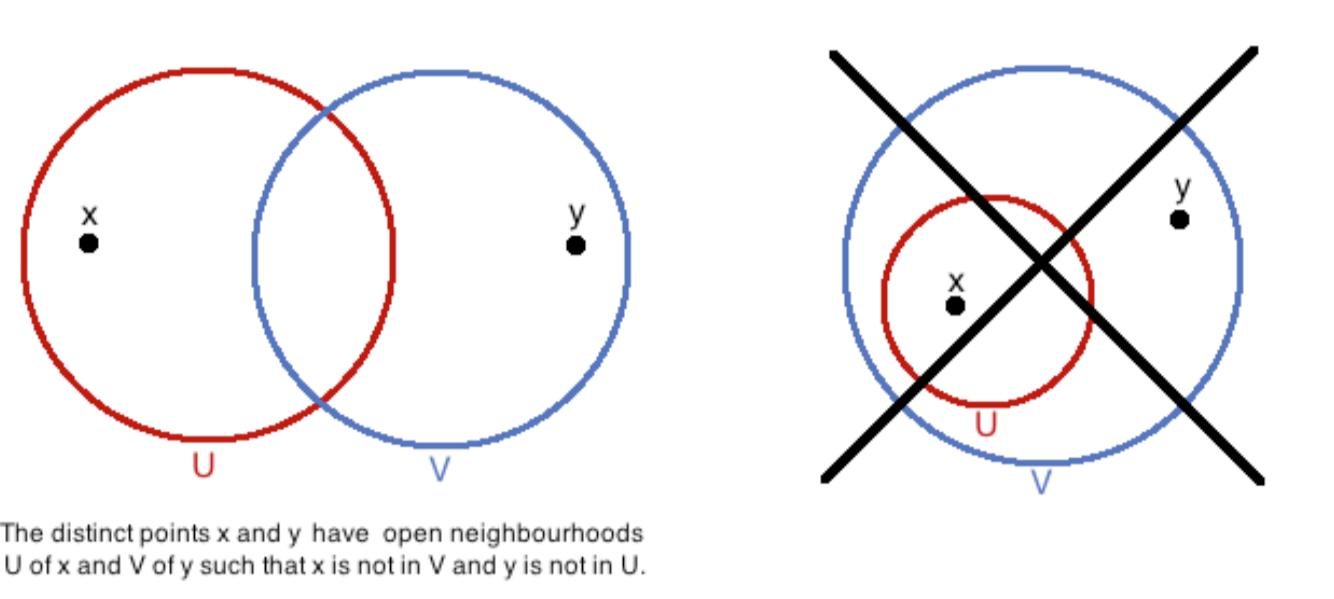
\includegraphics[scale = 0.3]{fotos_topo_1/t1.jpeg}
\end{equation}
Els diferents punts $x$ i $y$ tenen diferents entorns oberts $U$ de $x$ i $V$ de $y$ tal que $x$ no és a $V$ ni $y$ a $U$.

\begin{ej}
\label{ej:frechet1} Si $X = \{a,b,c,d\}$ i $\tau$ és la topologia discreta, aleshores $X$ és $T_1$. Això és perquè $\forall x,y\in  X$, els entorns oberts $U = \{x\}$ i $V=\{y\}$ de $x$ i $y$ respectivament, satisfan que $x\not\in V$ i $y\not\in U$.
\end{ej}

\begin{ter}
\label{ter:t1implicat0} Si un espai topològic $X$ és $T_1$, aleshores també és $T_0$. És a dir, $T_1\Rightarrow T_0$.
\end{ter}
\begin{proof}
Suposem que $X$ és $T_1$ i siguin $x,y\in X$, $x\not=y$. Aleshores, com $X$ és $T_1$, $\exists$ entorns oberts $U$ de $x$ i $V$ de $y$ tal que $x\not\in V$ i $y\not\in U$. Aleshores se satisfà que $x\not\in V$ o bé $y\not\in U$.
\end{proof}

\begin{ej}
\label{ej:frechet2} Sigui $(X,d)$ un espai mètric i siguin $x,y\in X$. Posem $r = d(x,y)$ i trobem que $x\not\in B_r(y)$ i $y\not\in B_r(x)$. Per tant, tot espai topològic que provè d'un espai mètric és de Fréchet.
\end{ej}

\begin{ej}
\label{ej:frechet3} Sigui $\mathbb{R}$ amb la topologia següent:
\begin{equation}
    \notag
    \tau = \{\emptyset,\mathbb{R}\}\cup\{\mathbb{R}\setminus X\;:\;X\;\text{finit}\} 
\end{equation}
(la topologia dels complements finits). Aleshores, si $x,y\in \mathbb{R}$ són diferents, $\mathbb{R}\setminus\{y\}\in\tau$ i $y\not\in \mathbb{R}\setminus\{y\}$ i $x\in\mathbb{R}\setminus\{y\}$, i també $x\not\in\mathbb{R}\setminus\{x\}$ i $x\in\mathbb{R}\setminus\{y\}$, per tant és de Fréchet.
\end{ej}

\begin{prop}
\label{prop:frechet} Un espai topològic $X$ és de Fréchet si i només si tot singletó de $X$ (subconjunt de $X$ amb un sol element) és tancat en $X$.
\end{prop}
\begin{proof}
($\Rightarrow$) Suposem que $X$ és $T_1$. Sigui $x\in X$ i considerem el singletó $\{x\}$. Hem de provar que $\{x\}^c = X\setminus\{x\}$ és obert. Sigui $y\in X\setminus\{x\}$. Aleshores $x\not=y$. Com $X$ és de Fréchet, existeix un entorn obert $V$ de $y$ tal que $x\not\in V$. Però aleshores $V\subseteq X\setminus\{x\}$ i $y\in\left(\{x\}^c\right)^{o} = \left(X\setminus\{x\}\right)^{o}$ que prova que $X\setminus\{x\}$ és obert. Per tant, tot singletó $\{x\}$, amb $x\in X$, és tancat.

($\Leftarrow$) Suposem ara que tot singletó $\{x\}$ és tancat. Siguin $x,y\in X$ i suposem que $x\not=y$. Aleshores $\{x\}$ i $\{y\}$ són tancats. Sigui $U = \{y\}^c = X\setminus\{y\}$ i $V = \{x\}^c = X\setminus\{x\}$. Aleshores $U$ i $V$ són entorns oberts de $x$ i $y$ respectivament, satisfent que $y\not\in U$ i $x\not\in V$. Per tant $X$ és $T_1$.
\end{proof}

\begin{nota}
\label{nota:frechet} No tot espai topològic és de Fréchet. Per exemple, si $X$ té més d'un punt i $\tau$ és la topologia grollera, aleshores $(X,\tau)$ no és de Fréchet, atès que els seus punts no són tancats (punts aquí vol dir singletons, és a dir, conjunts que contenen només un punt). 
\end{nota}

Observem que és clar que un espai homeomorf a un espai de Fréchet és de Fréchet. En canvi, la imatge per una aplicació contínua d'un espai de Fréchet no és, en general, de Fréchet. Per exemple, sigui $X$ amb més d'un punt i sigui $\tau_d$ la topologia discreta i $\tau_g$ la topologia grollera. Aleshores,
\begin{equation}
    \notag
    \begin{array}{rl}
        id:(X,\tau_d) & \longrightarrow (X,\tau_g) \\
        x & \longmapsto x
    \end{array}
\end{equation}
és contínua i $(X,\tau_d)$ és $T_1$, però $(X,\tau_g)$ no.

\section{Espais topològics de Hausdorff}

\begin{defi}
[Espai de Hausdorff]\label{def:hausdorff}\index{Hausdorff}\index{Espai topològic de Hausdorff} Sigui $(X,\tau)$ un espai topològic. Si per tot $x,y\in X$, $x\not=y$, existeixen entorns oberts $U_x$ i $U_y$ respectivament, tals que $x\in U_x$ i $y\in U_y$ però $U_x\cap U_y = \emptyset$, aleshores $(X,\tau)$ es diu que és de \textit{Hausdorff} o $T_2$
\end{defi}

Essencialment, $(X,\tau)$ és de Hausdorff si podem separar cada element de $X$ amb entorns oberts disjunts com il·lustra la imatge:
\begin{equation}
    \notag
    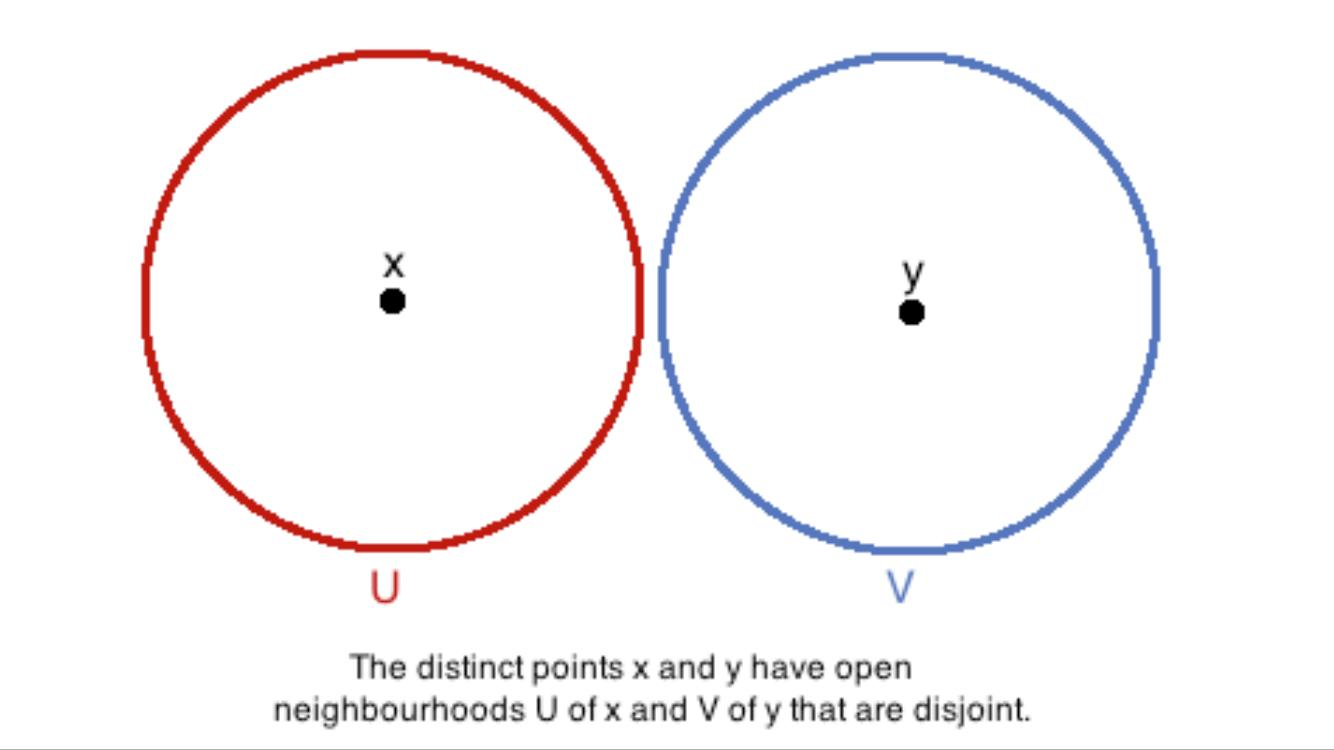
\includegraphics[scale = 0.3]{fotos_topo_1/t2.jpeg}
\end{equation}

\begin{ter}
\label{ter:t2implicat1} Si $X$ és un espai topològic de Hausdorff, aleshores també és de Fréchet.
\end{ter}
\begin{proof}
Sigui $X$ un espai topològic $T_2$ i siguin $x,y\in X$, $x\not=y$. Com $X$ és $T_2$, $\exists U_x, U_y$ entorns oberts de $x$ i $y$ respectivament, tals que $U_x\cap U_y = \emptyset$. Aleshores, en particular, $y\not\in U_x$ i $x\not\in U_y$ i per tant $X$ és $T_1$.
\end{proof}

\begin{nota}
En general, no tot espai de Fréchet és de Hausdorff. Per exemple, considerem un conjunt $X$ infinit dotat de la topologia dels complements finits
\begin{equation}
    \notag
    \tau = \{U\subset X\;:\;U^c\;\text{és finit o bé}\;U = \emptyset\}\cup\{X\}
\end{equation}
Siguin $x,y\in X$ amb $x\not=y$. Considerem els conjunts $U = X\setminus \{x\}$ i $V = X\setminus\{y\}$. Aleshores $U$ i $V$ són entorns oberts de $x$ i $y$ respectivament i $x\not\in V$ ni $y\not\in U$. Per tant $X$ és un espai de Fréchet.

Però per altra banda, tot entorn obert de $x$ és de la forma $U\setminus\{x_1,x_2,\ldots,x_n\}$, on $x\not=x_i$, $\forall i\in\{1,\ldots,n\}$ i anàlogament, els entorns de $y$ són de la forma $V = X\setminus\{y_1,\ldots,y_m\}$, amb $y\not=y_j$, $\forall j\in\{1,\ldots,m\}$. En qualsevol cas tenim $U\cap V = \not=\emptyset$, per tant no pot ser $T_2$.
\end{nota}

\begin{ej}
\label{ej:hausdorff1} Potser l'exemple més familiar d'espais de Hausdorff és $(\mathbb{R},\tau)$ on $\tau$ és la topologia usual d'intervals oberts a $\mathbb{R}$. Per provar que aquest espai topològic és de Hausdorff, siguin $x,y\in X$, $x\not=y$, i sense pèrdua de generalitat, suposem $x<y$. La distància euclidiana entre $x$ i $y$ és $d(x,y) = |x-y|$. Ara, siguin
\begin{equation}
    \notag
    U = \left(x-\frac{d(x,y)}{2},x+\frac{d(x,y)}{2}\right),\qquad V = \left(y-\frac{d(x,y)}{2},y+\frac{d(x,y)}{2}\right)
\end{equation}
\begin{equation}
    \notag
    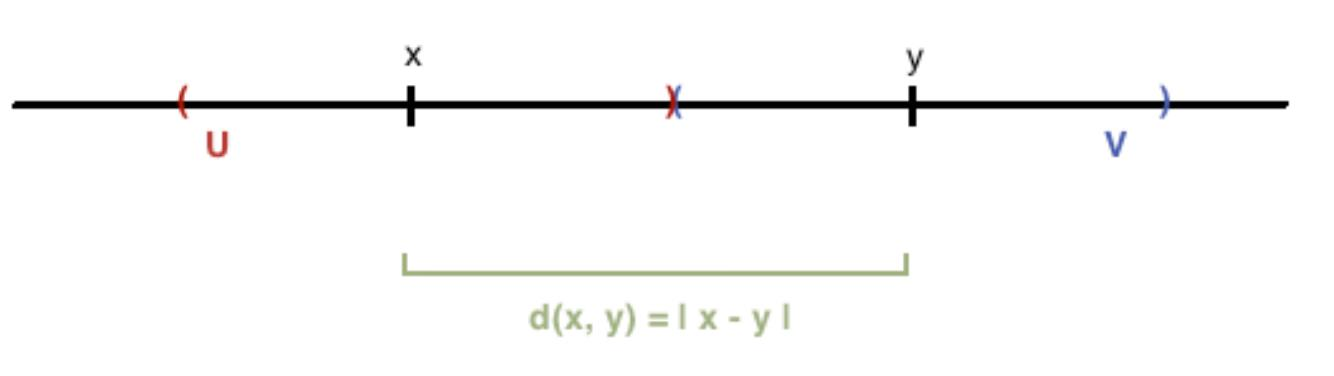
\includegraphics[scale = 0.3]{fotos_topo_1/hausdorffexemple1.jpeg}
\end{equation}
Aleshores $U,V\in \tau$ i $U\cap V= \emptyset$. Però $x,y\in X$ són arbitràries, per tant això se satisfà $\forall x,y\in X$, $x\not=y$. Per tant, $(\mathbb{R},\tau_e)$ és un espai de Hausdorff ( també de Fréchet, per (\ref{ter:t2implicat1})).
\end{ej}

\begin{ej}
\label{ej:hausdorff2} Generalitzem l'exemple 1 a espais mètrics qualssevol. Donat un espai mètric $(X,d)$ prenem $x,y\in X$ diferents i definim $r = \frac{1}{2}d(x,y)$. Aleshores $x\in B_r(x)$ i $y\in B_r(y)$ però $B_r(x)\cap B_r(y) = \emptyset$.
\end{ej}

\begin{ej}
\label{ej:hausdorff3} Sigui $X\not=\emptyset$ i $\tau$ la topologia discreta a $X$. Aleshores, $\forall x,y\in X$, $x\not=y$, tenim que $\{x\},\{y\}\in\tau$. Si diem $U = \{x\}$ i $V = \{y\}$ obtenim que $x\in U$, $y\in V$ i que $U\cap V = \emptyset$. Per tant $(X,\tau)$ és de Hausdorff.
\end{ej}

\begin{ej}
\label{ej:hausdorff4} Considerem $X = \{a,b,c,d\}$ i 
\begin{equation}
    \notag
    \tau = \{\emptyset,\{a\},\{b\},\{a,b\},\{b,c\},\{a,b,c\},X\} .
\end{equation}
Veiem si $(X,\tau)$ és de Hausdorff.

Notem que per $d\in X$, l'únic entorn obert possible és $X$. D'altra banda, però, per a $a\in X$, tenim que els seus entorns oberts són $\{a\}$, $\{a,b\}$, $\{a,b,c\}$ i $X$, i per tots aquests conjunts, la intersecció amb $X$ no és buida. Per tant $(X,\tau)$ no és de Hausdorff.
\end{ej}

\begin{ej}
\label{ej:hausdorff5} Sigui $X$ un conjunt no buit i $\tau_g$ la topologia grollera, $\tau_g = \{\emptyset,X\}$. Aleshores, $\forall x,y\in X$, $x\not=y$, tenim que els seus únics entorns possibles són $X$, per als dos, i aleshores $X\cap X = X\not=\emptyset$. Per tant no és de Hausdorff.
\end{ej}

\begin{ej}
\label{ej:hausdorff6} Considerem l'espai topològic $(\mathbb{R},\tau)$, on $\tau = \{(-n,n)\;:\;n\in\mathbb{N}\}$. Considerem els nombres $0,1/2\in\mathbb{R}$. Observem que
\begin{equation}
    \notag
    0,\frac{1}{2}\in (-1,1)\subset(-2,2)\subset\cdots\subset(-n,n)\subset\cdots
\end{equation}
és a dir, tot obert de $\tau$ és un entorn obert per $0,\frac{1}{2}$. Així doncfs, si $U$ i $V$ són entorns de $0$ i $\frac{1}{2}$, respectivament, aleshores $U\cap V\not=\emptyset$. Per tant, $(\mathbb{R},\tau)$ no és de Hausdorff.
\end{ej}

\begin{ej}
\label{ej:hausdorff7} Considerem el conjunt $\mathbb{R}$ amb la topologia dels complements finits 
\begin{equation}
    \notag
    \tau = \{U\subseteq X\;:\;U = \emptyset\;\text{o bé $U^c$ és finit}\}
\end{equation}
És de Hausdorff?

Primer considerem qualsevol obert de $\mathbb{R}$ amb $\tau$. Mostrarem que cap obert és disjunt i, per tant, cap entorn serà disjunt. Siguin $U,V\in\tau$. Aleshores $U^c$ i $V^c$ són finits. Escrivim
\begin{equation}
    \notag
    U^c = \{x_1,\ldots,x_n\},\qquad V^c = \{y_1,\ldots,y_n\},\quad x_i,y_j\in\mathbb{R},\;\forall i,j.
\end{equation}
Per tant, 
\begin{equation}
    \notag
    U = \mathbb{R}\setminus\{x_1,\ldots,x_n\},\qquad V = \mathbb{R}\setminus\{y_1,\ldots,y_m\}
\end{equation}
i aleshores
\begin{equation}
    \notag
    U\cap V = (\mathbb{R}\setminus\{x_1,\ldots,x_n\})\cap (\mathbb{R}\setminus\{y_1,\ldots,y_m\}) = \mathbb{R}\setminus\{x_1,\ldots,x_n,y_1,\ldots,y_m\}
\end{equation}
Però $\{x_i,y_j\}_{i=1,\ldots,n;\;j=1,\ldots,m}$ és finit i per tant $U\cap V\not=\emptyset$ (és un obert de $\tau$). Per tant $(\mathbb{R},\tau)$ no pot ser de Hausdorff.
\end{ej}

\begin{prop}
\label{prop:hausdorff1}\label{ej:hausdorff8} Si $(X,\tau)$ és de Hausdorff, aleshores qualsevol successió $\{x_n\}_{n=1}^\infty$ en $X$ convergeix com a màxim a un punt $x\in X$.
\end{prop}
\begin{proof}
Suposem que $x,y\in X$, $x\not=y$, i sigui $(x_n)_n$ una successió convergent a $x$. Com $(X,\tau)$ és de Hausdorff, tenim que $\exists U,V$, entorns oberts de $x$ i $y$ respectivament, tals que $U\cap V = \emptyset$. Com $(x_n)_{n=1}^\infty$ convergeix a $x$, $\exists n_0\in \mathbb{N}$ tal que $\forall n\geq n_0$, $x_n\in U$ (veure (\ref{def:successioconvergentesptopo})). Però com $U\cap V = \emptyset$, implica que aquests $x_n$ no estaran a $V$, per tant $(x_n)_n$ no convergeix a $y$.
\begin{equation}
    \notag
    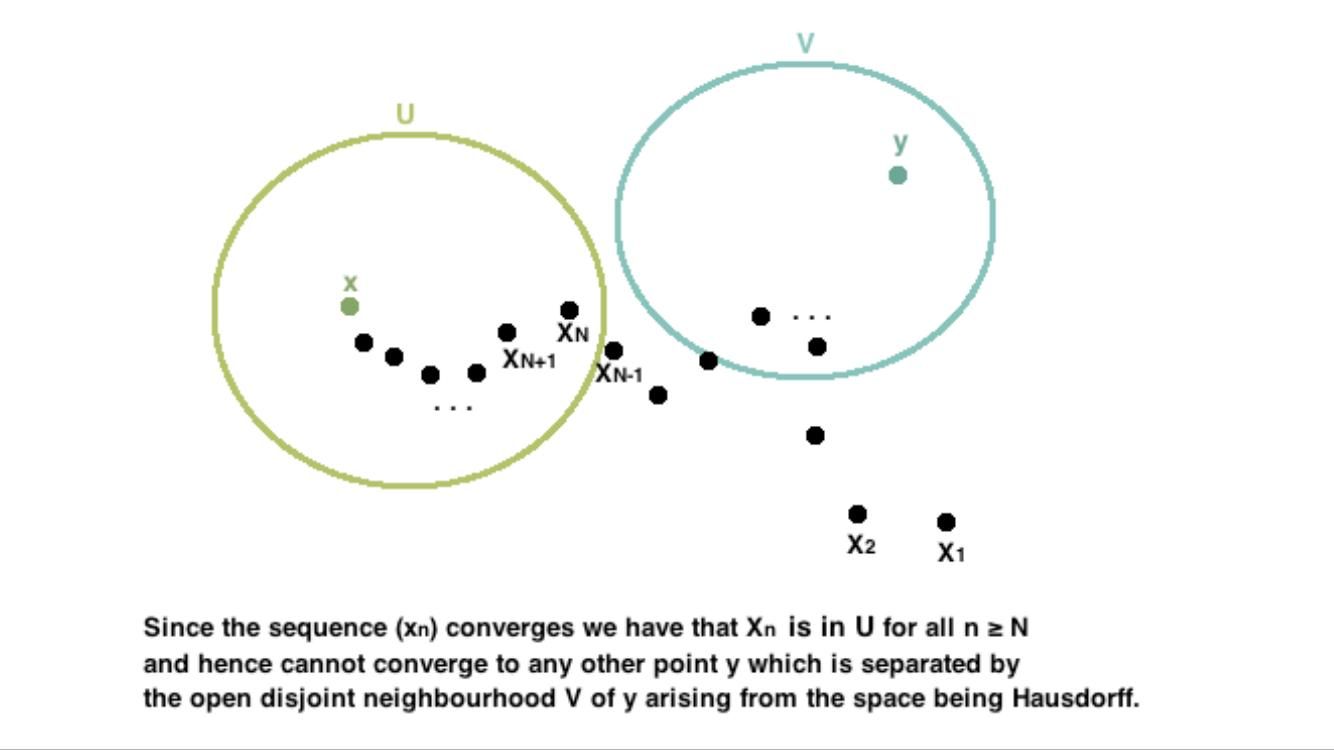
\includegraphics[scale = 0.3]{fotos_topo_1/hausdorffexemple8.jpeg}
\end{equation}
\end{proof}

\begin{prop}
\label{prop:hausdorff2} 
\begin{enumerate}[(1)]
    \item Un subespai topològic (subconjunt dotat de la topologia subespai, (\ref{def:subespaitopologic})) d'un espai de Hausdorff és de Hausdorff.
    \item El producte d'espais topològics de Hausdorff és de Hausdorff.
\end{enumerate}
\end{prop}
\begin{proof}
\begin{enumerate}[(1)]
    \item És equivalent a dir que la propietat 'ser de Hausdorff' és hereditària (recordem \ref{def:hereditaria}). És a dir, que si $(X,\tau)$ és de Hausdorff i $A\subseteq X$, aleshores, el subespai topològic $(A,\tau_A)$, on $\tau_A$ és la topologia subespai, és de Hausdorff.
    
    Siguin $x,y\in A$. Aleshores $x,y\in X$, ja que $A\subseteq X$. Com $X$ és de Hausdorff, $\exists U,V$ entorns oberts de $x$ i $y$ respectivament, tals que
    \begin{equation}
        \notag
        U\cap V = \emptyset
    \end{equation}
    Com $U$ i $V$ contenen $x$ i $y$ respectivament, tenim que $A\cap U$ i $A\cap V$ són entorns oberts de $x$ i de $y$ en $A$, respectivament. A més, veiem que 
    \begin{equation}
        \notag
        (A\cap U)\cap(A\cap V) = A\cap(U\cap V) = A\cap\emptyset = \emptyset
    \end{equation}
    Per tant, $\forall x,y\in A$, $x\not=y$, existeixen entorns oberts de $x$ i $y$ disjunts.
    
    \item Siguin $X$ i $Y$ dos espais de Hausdorff. Veiem que el producte $X\times Y$ és de Hausdorff. Si $(x_1,y_1),(x_2,y_2)\in X\times Y$ són punts diferents, aleshores alguna de les dues coordenades és diferent. Suposem, per exemple, que $x_1\not=x_2$, i siguin $U_1$ i $U_2$ dos oberts disjunts tals que $x_i\in U_i$, $i=1,2$. Aleshores, $V_i = U_i\times Y$ són dos oberts disjunts de $X\times Y$ tals que $(x_i,y_i)\in V_i$, per $i=1,2$.
\end{enumerate}
\end{proof}
Amb petites modificacions es prova el mateix resultat per a espais de Fréchet.

\begin{prop}
\label{prop:hausdorff3} Sigui $(X,\tau)$ un espai topològic i sigui
\begin{equation}
    \notag
    \Delta = \{(x,y)\in X\times X\;:\;y = x\}
\end{equation}
la diagonal. Aleshores $X$ és de Hausdorff si i només si $\Delta$ és tancat a $X\times X$.
\end{prop}
\begin{proof}
$\Delta$ és tancat si i només si tot punt $(x,y)\in X\times X\setminus\Delta$ és interior a $X\times X\setminus\Delta$. Com que els oberts de la forma producte d'oberts formen una base de la topologia producte, $(x,y)\in X\times X\setminus\Delta$ és interior si i només si existeixen oberts $U$ de $X$ i $V$ de $X$ tals que $(x,y)\in U\times V\subset X\times X\setminus \Delta$. Aquesta condició és equivalent a la de Hausdorff ja que
\begin{equation}
    \notag
    (U\times V)\cap \Delta = \{(x,x)\;:\;x\in U\times V\}
\end{equation}
\end{proof}

\section{Espais topològics regulars i normals}
\subsection{Espais topològics regulars}

\begin{defi}
[Espai regular]\label{def:regular}\index{Regular}\index{Espai topològic regular} Sigui $(X,\tau)$ un espai topològic. Diem que $X$ és \textit{regular} o $T_3$ si per a tot punt $p\in X$ i per a tot tancat $F$ de $X$ amb $p\not\in F$, existeixen oberts disjunts $U_1$ i $U_2$ tals que $p\in U_1$ i $F\subset U_2$.
\end{defi}
\begin{equation}
    \notag
    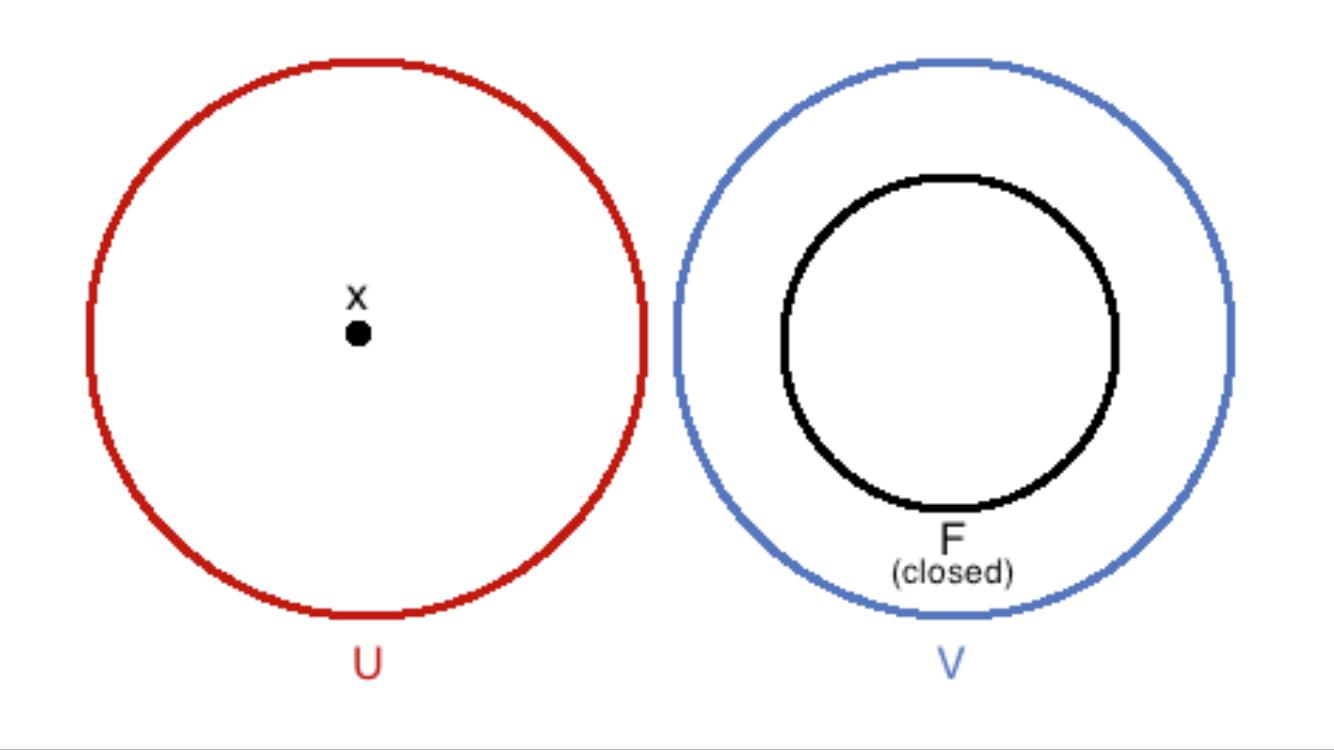
\includegraphics[scale = 0.3]{fotos_topo_1/t3.jpeg}
\end{equation}

\begin{ter}
\label{ter:regular} Si un espai topològic $X$ és regular, aleshores és també de Hausdorff. És a dir, $T_3\Rightarrow T_2$.
\end{ter}
\begin{proof}
Sigui $X$ un espai topològic regular. Aleshores, siguin $x,y\in X$, $x\not=y$. Com $T_3$ és també $T_1$ trivialment, tot singletó $\{x\}$ és tancat. Per tant, $\{x\}$ és tancat i $\{y\}$ també. Si diem $F = \{y\}$ ja tenim que existeix $U$ entorn obert de $x$ i $V$ de $F$ tals que $U\cap V = \emptyset$. Per tant, $X$ és $T_2$.
\end{proof}

\subsection{Espais topològics normals}

\begin{defi}
[Espai normal]\label{def:t3implicat2}\index{Normal}\index{Espai topològic normal} Sigui $(X,\tau)$ un espai topològic. Diem que $X$ és \textit{normal} o $T_4$ si per a tota parella $F_1,F_2$ de tancats disjunts de $X$, existeixen oberts disjunts $U_1$ i $U_2$ tals que $F_1\subset U_1$ i $F_2\subset U_2$.
\end{defi}

\begin{equation}
    \notag
    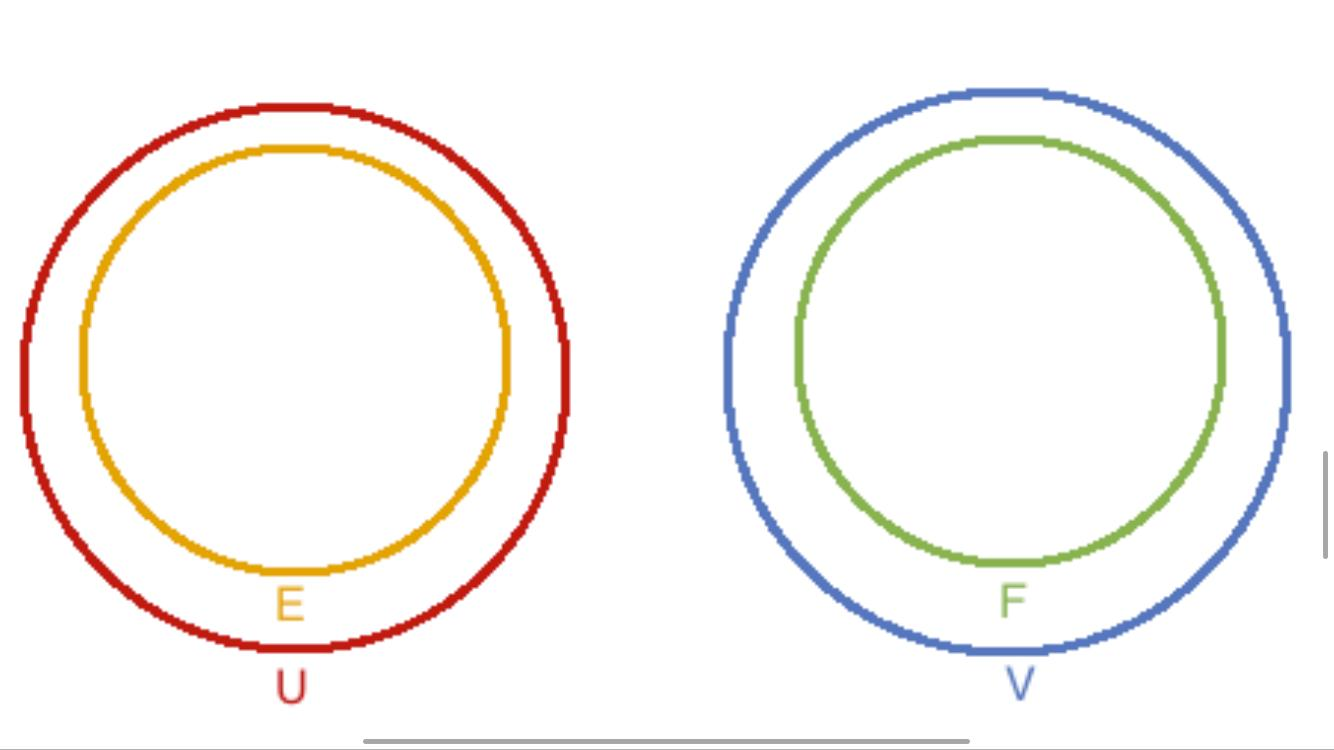
\includegraphics[scale = 0.3]{fotos_topo_1/t4.jpeg}
\end{equation}

\begin{ter}
\label{ter:t4implicat3} Si un espai topològic $X$ és normal, aleshores és també regular. És a dir, $T_4\Rightarrow T_3$.
\end{ter}
\begin{proof}
Sigui $X$ un espai $T_4$. Aleshores, hem de veure que és regular. Sigui $x\in X$ i $F$ un tancat de $X$ que no conté $x$. Com $T_4\Rightarrow T_1$ trivialment, tot singletó és tancat. Per tant, en particular, $\{x\}$ és tancat. Per tant, per ser $T_4$, existeixen entorns oberts $U_1$ i $U_2$ de $\{x\}$ i $F$ respectivament, que compleixen $U\cap V = \emptyset$.
\end{proof}

\subsection{Relació entre ells}

Als teoremes (\ref{ter:t1implicat0}), (\ref{ter:t2implicat1}), (\ref{ter:t3implicat2}) i (\ref{ter:t4implicat3}) hem vist la següent cadena d'implicacions:
\begin{equation}
    \label{eq:cadenaimplicacionsti}
    T_4 \Rightarrow T_3 \Rightarrow T_2 \Rightarrow T_1 \Rightarrow T_0.
\end{equation}

Veiem ara una caracterització dels espais topològics que provenen dels espais mètrics, que ens servirà com a exemple.

\begin{prop}
\label{prop:totespaimetricest4} Tot espai mètric (és a dir, espai topològic provinent d'un espai mètric) és normal i regular.
\end{prop}
\begin{proof}
Atès que tot espai mètric és de Fréchet, serà suficient provar que és normal. Siguin $F_1$ i $F_2$ tancats d'un espai mètric $(X,d)$ tals que $F_1\cap F_2 = \emptyset$. Sigui $x\in F_1$ i definim
\begin{equation}
    \notag
    r_x = \inf\{d(x,y)\;:\;y\in F_2\}\in[0,+\infty).
\end{equation}
Si $r_x = 0$, aleshores $\forall\varepsilon>0,\;\exists y\in F_2$ tal que $d(x,y)<\varepsilon$, és a dir, $F_2\cap B_\varepsilon(x)\not=\emptyset$. Anàlogament, es defineix un obert $U_2$ que conté $F_2$. Veiem, finalment, que $U_1\cap U_2 = \emptyset$. En efecte, si existís un $p\in U_1\cap U_2$, aleshores tindríem punts $x_1\in F_1$ i $x_2\in F_2$ tals que
\begin{equation}
    \notag
    p\in B_{\frac{r_{x_1}}{2}}(x_1)\cap B_{\frac{r_{x_2}}{2}}(x_2).
\end{equation}
Per definició, $d(x_1,x_2)\geq r_{x_i},\;i=1,2$. Així:
\begin{equation}
    \notag
    \frac{r_{x_1}}{2}+\frac{r_{x_2}}{2}\leq d(x_1,x_2)\leq d(x_1,p)+d(p,x_2)<\frac{r_{x_1}}{2}+\frac{r_{x_2}}{2},
\end{equation}
la qual cosa és absurda.
\end{proof}

\begin{lema}[Lema de Urysohn]
\label{lema:lemadeurysohn} Sigui $(X,\tau)$ un espai topològic. $X$ és normal si i només si per a tota parella $F_1,F_2$ de tancats disjunts de $X$ existeix una aplicació contínua
\begin{equation}
    \notag
    f:X\rightarrow [0,1]
\end{equation}
tal que $F_1 = f^{-1}(\{0\})$ i $F_2 = f^{-1}(\{1\})$.
\end{lema}

Finalment, cal destacar que les implicacions recíproques de la cadena d'implicacions (\ref{eq:cadenaimplicacionsti}) no són sempre certes. Ja vam veure que $T_1\not\Rightarrow T_2$. Es poden trobar contraexemples per veure que $T_2\not\Rightarrow T_3$ i $T_3\not\Rightarrow T_4$.



















































\end{document}